\documentclass{article}
\usepackage[paperwidth=44in, paperheight=34in, left=1in, right=1in, top=1in, bottom=1in]{geometry}

\usepackage{tikz}
\usepackage{tikz-qtree}
\usepackage{multirow}

\tikzset
{
  GenericNodeStyle/.style =
  {
    shape = rectangle,
    rounded corners = 2mm,
    scale = 1.0,
    thick,
  }
}

\begin{document}
\thispagestyle{empty}

\begin{center}
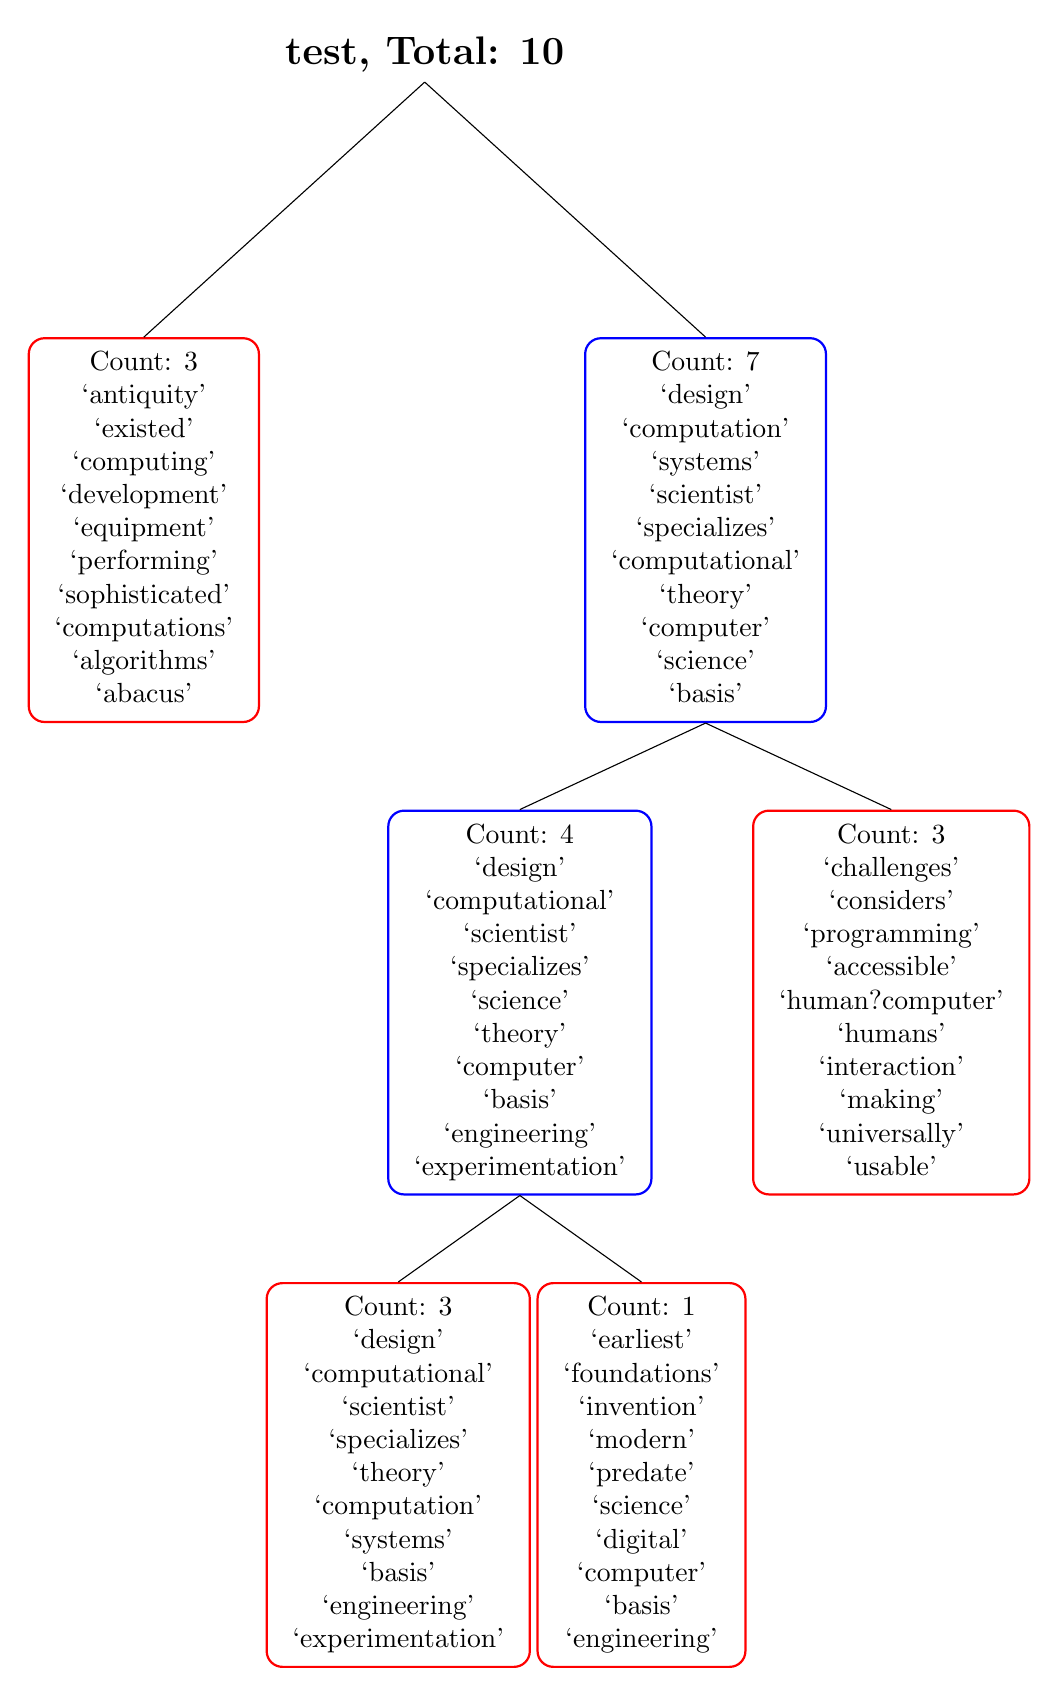
\begin{tikzpicture}[level distance=6cm]
  \Tree [.{\Large{\textbf{test, Total: 10}}}
    [
      .\node[GenericNodeStyle, draw=red] {
        \begin{tabular}{c}
        Count: 3 \\
        `antiquity' \\
        `existed' \\
        `computing' \\
        `development' \\
        `equipment' \\
        `performing' \\
        `sophisticated' \\
        `computations' \\
        `algorithms' \\
        `abacus' \\
        \end{tabular}
      };
    ]
    [
      .\node[GenericNodeStyle, draw=blue] {
        \begin{tabular}{c}
        Count: 7 \\
        `design' \\
        `computation' \\
        `systems' \\
        `scientist' \\
        `specializes' \\
        `computational' \\
        `theory' \\
        `computer' \\
        `science' \\
        `basis' \\
        \end{tabular}
      };
        [
          .\node[GenericNodeStyle, draw=blue] {
            \begin{tabular}{c}
            Count: 4 \\
            `design' \\
            `computational' \\
            `scientist' \\
            `specializes' \\
            `science' \\
            `theory' \\
            `computer' \\
            `basis' \\
            `engineering' \\
            `experimentation' \\
            \end{tabular}
          };
            [
              .\node[GenericNodeStyle, draw=red] {
                \begin{tabular}{c}
                Count: 3 \\
                `design' \\
                `computational' \\
                `scientist' \\
                `specializes' \\
                `theory' \\
                `computation' \\
                `systems' \\
                `basis' \\
                `engineering' \\
                `experimentation' \\
                \end{tabular}
              };
            ]
            [
              .\node[GenericNodeStyle, draw=red] {
                \begin{tabular}{c}
                Count: 1 \\
                `earliest' \\
                `foundations' \\
                `invention' \\
                `modern' \\
                `predate' \\
                `science' \\
                `digital' \\
                `computer' \\
                `basis' \\
                `engineering' \\
                \end{tabular}
              };
            ]
        ]
        [
          .\node[GenericNodeStyle, draw=red] {
            \begin{tabular}{c}
            Count: 3 \\
            `challenges' \\
            `considers' \\
            `programming' \\
            `accessible' \\
            `human?computer' \\
            `humans' \\
            `interaction' \\
            `making' \\
            `universally' \\
            `usable' \\
            \end{tabular}
          };
        ]
    ]
  ]
;
\end{tikzpicture}
\end{center}

\end{document}
